% Synderm modernization and Figure 3 update, October 2026.   pdflatex synderm_update.tex (twice)
\documentclass[aspectratio=169,11pt]{beamer}
\usetheme{default}
\usecolortheme{dove}
\setbeamertemplate{navigation symbols}{}
\setbeamertemplate{footline}[frame number]
\setbeamertemplate{itemize items}[circle]
\setbeamerfont{frametitle}{series=\bfseries,size=\large}
\setbeamercolor{frametitle}{fg=black}
\setbeamersize{text margin left=0.8cm,text margin right=0.8cm}
\usepackage{booktabs,graphicx,xcolor}
\graphicspath{{fig/}}
\newcommand{\muted}[1]{{\color{gray}\footnotesize #1}}

\title{Synderm: modernized package and new Figure 3 arms}
\subtitle{Status, 29 October 2026}
\author{}
\date{}

\begin{document}

\begin{frame}
  \titlepage
\end{frame}

% ---------------------------------------------------------------- 1. package
\begin{frame}{Modernizing the \texttt{synderm} package (v0.2, branch \texttt{modernize})}
  \begin{columns}[T]
    \column{0.47\textwidth}
    \textbf{Replaced}
    \begin{itemize}
      \item Stable Diffusion 2.1-base text-to-image \muted{(official weights no longer downloadable)}
      \item Stable Diffusion 1.5 inpainting (inpaint, in-then-outpaint)
      \item Two custom DreamBooth training loops, diffusers 0.31
    \end{itemize}
    \column{0.5\textwidth}
    \textbf{Now}
    \begin{itemize}
      \item Three generators behind one interface: \textbf{Qwen-Image-2.1}, \textbf{FLUX 3 Klein}, \textbf{SDXL} (+ SDXL inpainting)
      \item Text-to-image and reference-image edit; hard-mask inpaint via SDXL
      \item LoRA fine-tuning through \textbf{vendored upstream diffusers DreamBooth scripts} (pinned commit; text-to-image and image-to-image)
    \end{itemize}
  \end{columns}
  \vspace{1em}
  \muted{The code that produced the paper is untouched in \texttt{paper\_experiments/}; \texttt{main} still reproduces the published results.}
\end{frame}

% ---------------------------------------------------------------- 2. planned updates
\begin{frame}{Planned update to the paper: Figure 3 with current generators}
  \begin{itemize}
    \item Figure 3: nine-way accuracy vs. number of real training images per class, with and without 10 synthetic images per real
    \item The published SD arms stay as they are; new arms are added under the same classifier protocol
  \end{itemize}
  \vspace{0.6em}
  \begin{center}
  \begin{tabular}{lll}
    \toprule
    Generator & Adaptation & Methods \\
    \midrule
    \textbf{Qwen-Image-2.1} (open weights) & one LoRA per class & text-to-image, edit \\
    \textbf{GPT Image 2.5 Sunburst} (OpenAI) & none, zero-shot & edit \\
    \textbf{Nano Banana 2.1} (Google) & none, zero-shot & edit \\
    \bottomrule
  \end{tabular}
  \end{center}
  \vspace{0.6em}
  \begin{itemize}
    \item Proprietary models cannot be fine-tuned, so they run zero-shot from a reference image
    \item Five new random seeds; real-only baselines are rerun with the same seeds
  \end{itemize}
\end{frame}

% ---------------------------------------------------------------- 3. experiment overview
\begin{frame}{Figure 3 experiment: one run}
  \begin{enumerate}
    \item Sample $n$ real images per class from the training pool, $n \in \{1, 8, 16, 32, 64, 128, 228\}$
    \item Attach the \textbf{10 synthetic images} that belong to each sampled real image
      \begin{itemize}
        \item edit: generated \emph{from} that real image as the reference
        \item text-to-image: generated from the class prompt alone; the real image only names the files
      \end{itemize}
    \item Train EfficientNetV2-M (fastai, 224 px, early stopping on a 40-per-class validation split), with or without image transforms
    \item Score top-1 accuracy on the \textbf{360-image held-out test set} (40 per class)
  \end{enumerate}
  \vspace{0.6em}
  \begin{itemize}
    \item Arms: real only; real + 10 synthetic (edit); real + 10 synthetic (text-to-image)
    \item 7 sizes $\times$ 2 transform settings $\times$ 5 seeds = 70 runs per arm
    \item Synthetic images are generated once for \emph{every} pool image, so any sampled subset is covered
  \end{itemize}
\end{frame}

\begin{frame}{Figure 3 experiment: the data}
  \begin{columns}[T]
    \column{0.54\textwidth}
    \small
    \textbf{Fitzpatrick 17k, ``clean 10-label'' split}
    \begin{itemize}
      \item Training pool: 3{,}530 images, 10 labels
      \item The paper keeps the \textbf{nine most common labels}; folliculitis (191 images) is dropped: \textbf{3{,}339 images}
      \item Held-out test: 40 per label, never used for training or generation
      \item Validation: 40 per label drawn from the pool for each seed
      \item $n_{\max} = 228$: smallest class (272) minus validation
    \end{itemize}
    \textbf{Generator fine-tuning corpus}
    \begin{itemize}
      \item One LoRA per class, trained on \emph{all} pool images of that class (272 to 584), as the paper's per-class DreamBooth did
    \end{itemize}
    \column{0.42\textwidth}
    \small
    \begin{tabular}{lr}
      \toprule
      Label & Pool images \\
      \midrule
      psoriasis & 584 \\
      squamous cell carcinoma & 440 \\
      lichen planus & 412 \\
      basal cell carcinoma & 406 \\
      allergic contact dermatitis & 358 \\
      lupus erythematosus & 297 \\
      sarcoidosis & 286 \\
      neutrophilic dermatoses & 284 \\
      photodermatoses & 272 \\
      \midrule
      total & 3{,}339 \\
      \bottomrule
    \end{tabular}
  \end{columns}
\end{frame}

% ---------------------------------------------------------------- 4. proprietary: screen, samples, pilot
\begin{frame}{Zero-shot screen: real images vs. three generators (psoriasis)}
  \begin{center}
    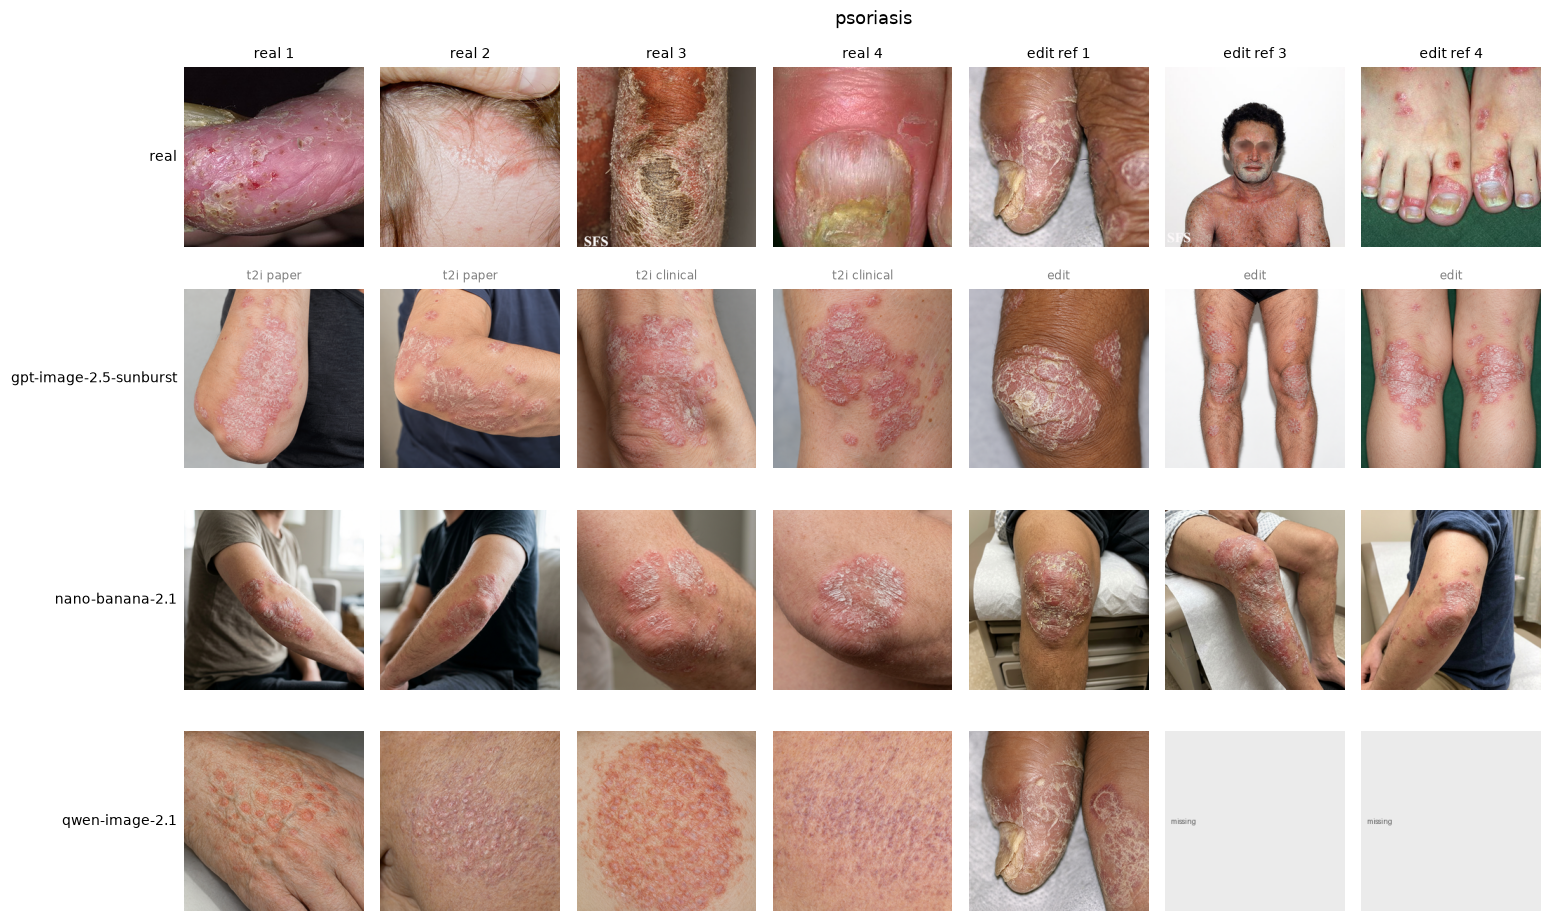
\includegraphics[height=0.72\textheight]{screen_psoriasis.png}
  \end{center}
  \muted{Left four columns: text-to-image from the paper's prompt and a clinical prompt. Right three: edits of the real reference above. Grey = refused or errored.}
\end{frame}

\begin{frame}{Proprietary edits: GPT Image 2.5 Sunburst vs. Nano Banana 2.1 (lichen planus)}
  \begin{center}
    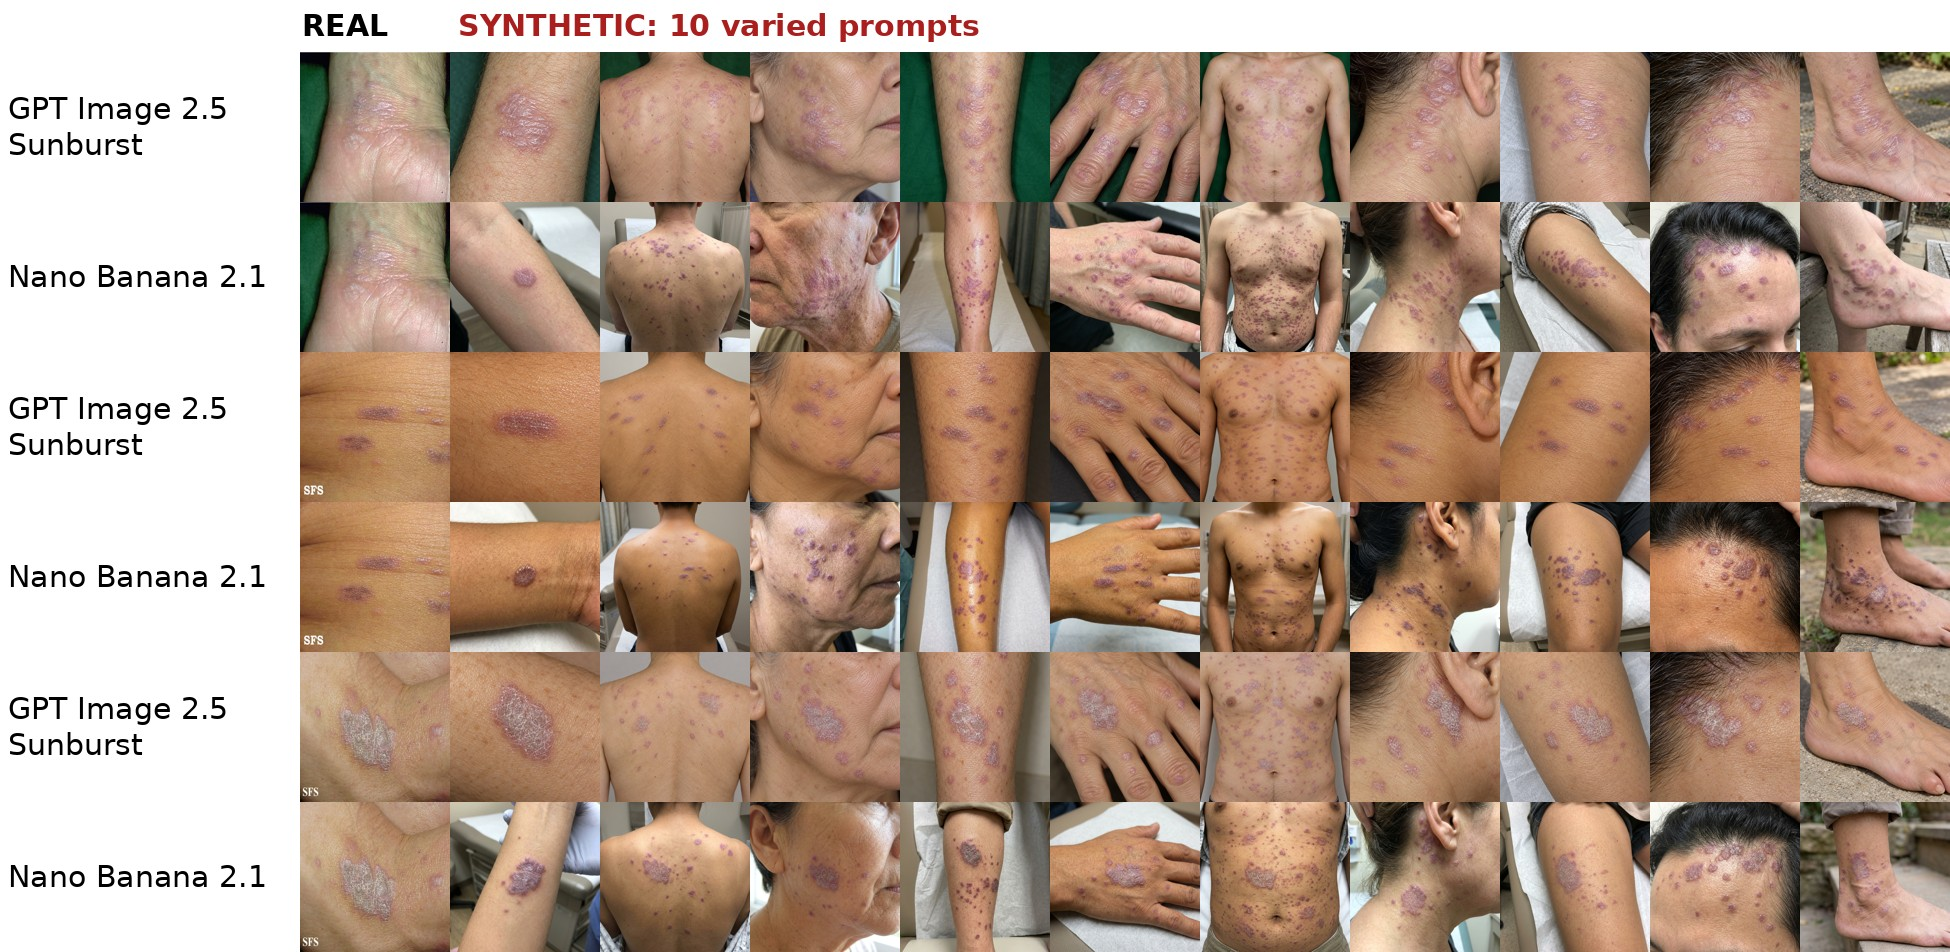
\includegraphics[height=0.70\textheight]{gpt_vs_nano_lichen.jpg}
  \end{center}
  \muted{Three reference images (left column), each edited 10 times with the 10 varied prompts. For each reference: GPT Image row above, Nano Banana row below.}
\end{frame}

\begin{frame}{One prompt vs. 10 prompts}
  \begin{center}
    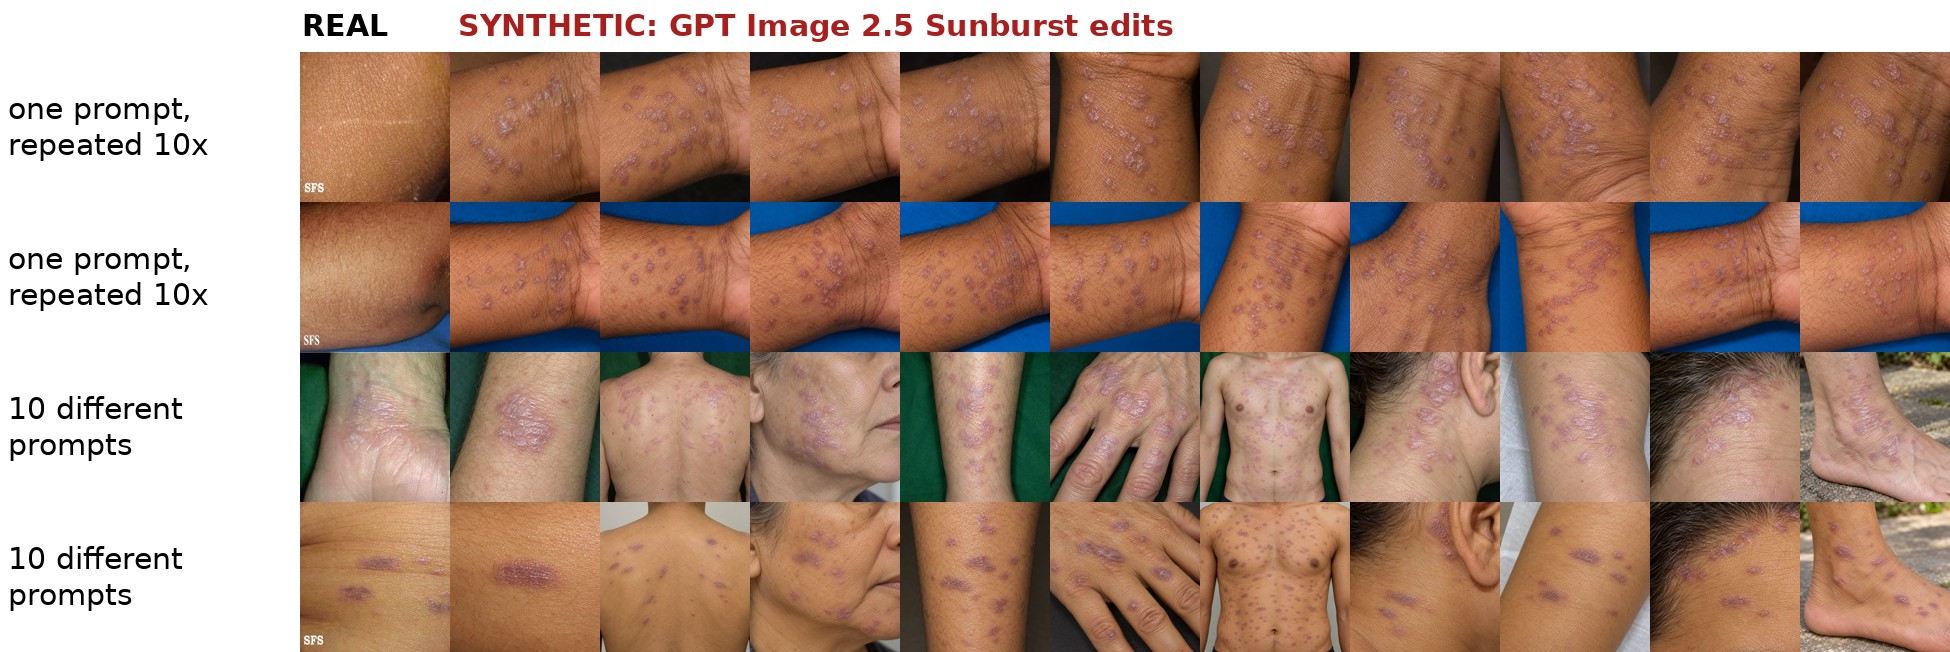
\includegraphics[height=0.62\textheight]{gpt_single_vs_varied_lichen.jpg}
  \end{center}
  \begin{itemize}
    \item One prompt repeated: nearly the same picture 10 times. Ten prompts (body site, framing, lighting): the pilot uses these
  \end{itemize}
\end{frame}

\begin{frame}{Preliminary results: proprietary models, zero-shot edits}
  \begin{columns}[T]
    \column{0.56\textwidth}
    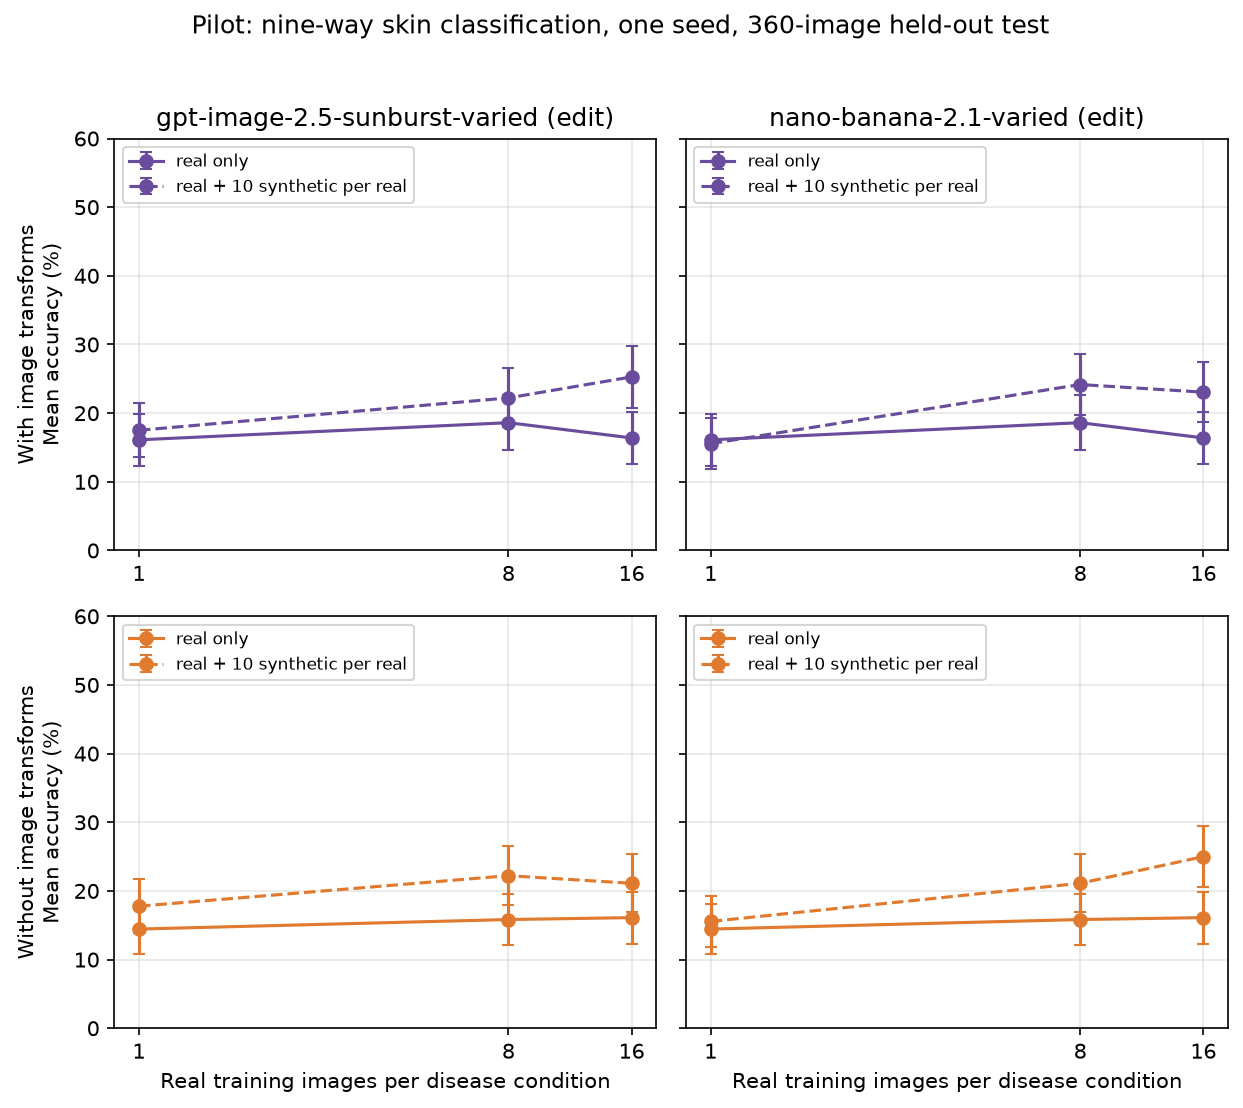
\includegraphics[width=\textwidth]{figure3_pilot.png}
    \column{0.42\textwidth}
    \vspace{1em}
    \small
    \begin{itemize}
      \item One seed, $n \in \{1, 8, 16\}$, 10 edits per real with the 10 varied prompts
      \item GPT Image 2.5 Sunburst (medium): \$0.019 per edit; 97 of 1{,}440 refused, replaced by extra edits of other references
      \item Nano Banana 2.1 (1K): \$0.034 per edit; 7 refused
      \item At $n = 16$: 25\% vs. 16\% real-only (GPT, with transforms); 25\% vs. 16\% (Nano Banana, without)
      \item Wide intervals: 360 test images, one seed
    \end{itemize}
  \end{columns}
\end{frame}

% ---------------------------------------------------------------- 5. fine-tuned qwen, text-to-image
\begin{frame}{Fine-tuned Qwen-Image-2.1, text-to-image: training}
  \begin{columns}[T]
    \column{0.42\textwidth}
    \begin{itemize}
      \item One LoRA per class: rank 16, lr $10^{-4}$, 512 px, 2{,}000 steps, checkpoints every 500
      \item Caption: the paper's prompt, ``An image of \{condition\}, a skin disease''
      \item 33 min per class on one RTX PRO 6000; all nine trained
      \item Generation: one prompt, 10 seeds per real, 40 steps, 2.8 s per image
    \end{itemize}
    \column{0.55\textwidth}
    \muted{Untuned Qwen: real image on the left, then 10 seeds}\\
    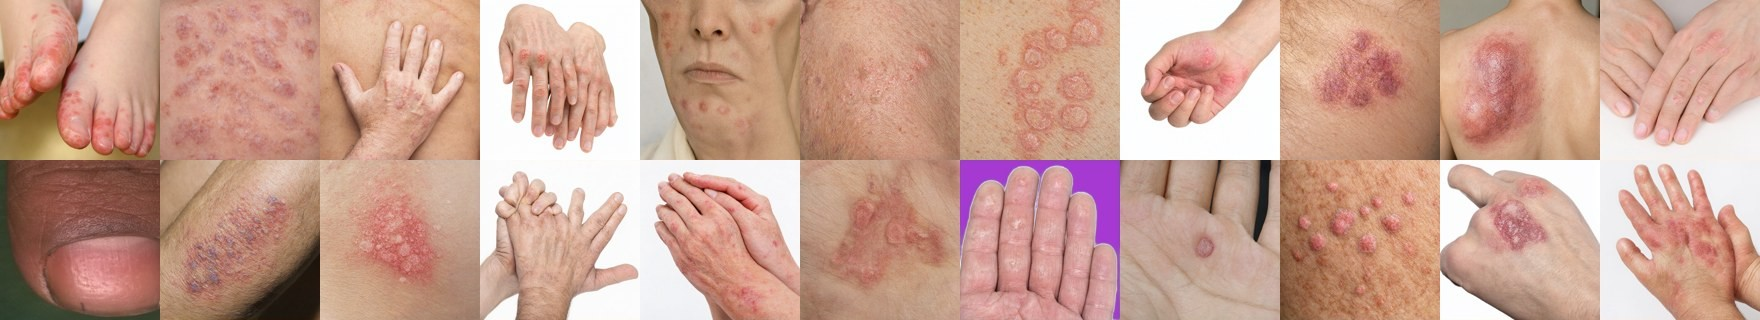
\includegraphics[width=\textwidth]{grid_t2i_untuned_psoriasis.jpg}\\[0.4em]
    \muted{Qwen + psoriasis LoRA, step 1500: same reals, 10 seeds}\\
    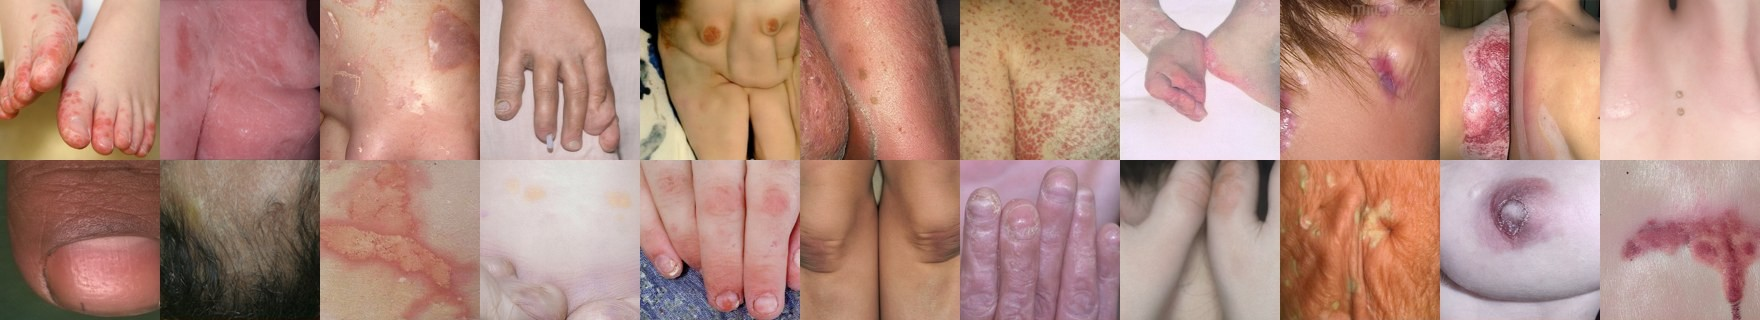
\includegraphics[width=\textwidth]{grid_t2i_ckpt1500_psoriasis.jpg}
  \end{columns}
\end{frame}

\begin{frame}{Fine-tuned Qwen-Image-2.1, text-to-image: does the LoRA help?}
  \begin{columns}[T]
    \column{0.5\textwidth}
    \textbf{Psoriasis pilot} \muted{(16 reals $\times$ 10 images; real-only DINOv2 probe)}
    \begin{center}
    \begin{tabular}{lcc}
      \toprule
      & label match & variety \\
      \midrule
      untuned Qwen & 0.49 & 0.37 \\
      LoRA, step 500 & 0.68 & 0.55 \\
      LoRA, step 1000 & 0.63 & 0.51 \\
      \textbf{LoRA, step 1500} & \textbf{0.78} & \textbf{0.53} \\
      LoRA, step 2000 & 0.66 & 0.54 \\
      GPT Image edits (varied) & 0.89 & 0.43 \\
      \muted{random sets of 10 reals} & & 0.59 \\
      \bottomrule
    \end{tabular}
    \end{center}
    \column{0.47\textwidth}
    \vspace{0.5em}
    \small
    \begin{itemize}
      \item Label match: share of images a probe trained on real images only assigns to the class (relative measure)
      \item Variety: mean DINOv2 distance among the 10 images of one real
      \item Confirmed on two more classes: basal cell carcinoma 0.76 vs. 0.16 untuned, lupus 0.40 vs. 0.16
      \item The LoRA picks up the dataset's look (varied sites, clinic backgrounds, darker skin tones) and its artifacts
    \end{itemize}
  \end{columns}
\end{frame}

\begin{frame}{Where the variety among the 10 images comes from: seeds vs. prompts}
  \begin{columns}[T]
    \column{0.46\textwidth}
    \small
    \begin{itemize}
      \item \textbf{Seeds} (Qwen): one prompt, 10 seeds. With the LoRA the spread among the 10 images (0.53) is close to that of 10 random real images (0.59); untuned Qwen gives mostly hands on white (0.37)
      \item \textbf{Prompts} (APIs expose no seed): 10 prompt variations change body site, framing and lighting; used for GPT Image and Nano Banana, and for Qwen edits, where one prompt returned near-copies of the reference
      \item Prompt variety is held in reserve for Qwen text-to-image; seed variety was enough
    \end{itemize}
    \column{0.52\textwidth}
    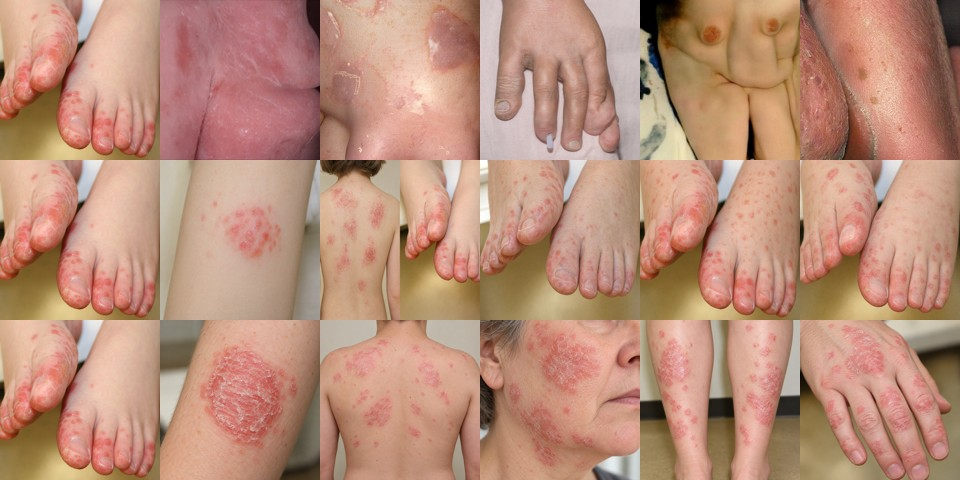
\includegraphics[width=\textwidth]{seed_vs_prompt_psoriasis.jpg}\\
    \muted{Same real image (left). Top: Qwen LoRA text-to-image, one prompt, five seeds. Middle: untuned Qwen edit, five prompts. Bottom: GPT Image edit, five prompts.}
  \end{columns}
\end{frame}

\begin{frame}{Status: the Qwen Figure 3 run is in progress}
  \begin{itemize}
    \item All nine text-to-image LoRAs are trained
    \item Generation of 10 synthetic images per training-pool image is running on 2$\times$ RTX PRO 6000: 33{,}390 text-to-image and 33{,}390 edit images, about 3 s per image
    \item The full Figure 3 sweep follows: $n \in \{1, 8, 16, 32, 64, 128, 228\}$, real only vs. + Qwen text-to-image vs. + Qwen edit, with and without image transforms, five seeds
    \item No API spend in this round: Qwen runs locally
  \end{itemize}
\end{frame}

\end{document}
